\documentclass[12pt]{article}
\usepackage{fullpage,enumitem,amsmath,amssymb,graphicx}
\usepackage{listings}
\usepackage{tikz}
\usepackage{hyperref}

\begin{document}

\begin{center}
{\Large CS 228 Winter 2018 Homework 2}

\begin{tabular}{rl}
SUNet ID: & 05794739 \\
Name: & Luis Perez \\
Collaborators: & \\
Late Days: & 2
\end{tabular}
\end{center}

By turning in this assignment, I agree by the Stanford honor code and declare
that all of this is my own work.

\section*{Problem 1}

\begin{enumerate}[label=(\alph*)]
  \item We can draw the network as follows. We first note that $(A \perp C \mid B) \land (A \perp D \mid B, C) \implies A \perp C,D \mid B)$ (similarly, we can collaps $A \perp D \mid B \land A \perp C \mid B,D \implies A \perp (C,D) \mid B$). We therefore know that observing $B$ must ``block'' any paths from $A$ to both $C$ and $D$. Furthermore, we know that $B \perp D$ and $A \perp D$, so we cannot have $B,D$ or $A,D$ connected. This leads us to the candidate network in Figure \ref{fig:bayesian_perfect_map}. 

  \begin{figure}[!h]
  	\centering
		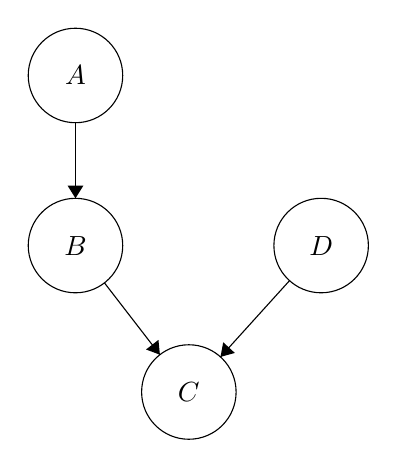
\begin{tikzpicture}[scale=0.2]
		\tikzstyle{every node}+=[inner sep=0pt]
		\draw [black] (27.3,-12.9) circle (3);
		\draw (27.3,-12.9) node {$A$};
		\draw [black] (27.3,-23.7) circle (3);
		\draw (27.3,-23.7) node {$B$};
		\draw [black] (34.5,-33) circle (3);
		\draw (34.5,-33) node {$C$};
		\draw [black] (42.9,-23.7) circle (3);
		\draw (42.9,-23.7) node {$D$};
		\draw [black] (27.3,-15.9) -- (27.3,-20.7);
		\fill [black] (27.3,-20.7) -- (27.8,-19.9) -- (26.8,-19.9);
		\draw [black] (29.14,-26.07) -- (32.66,-30.63);
		\fill [black] (32.66,-30.63) -- (32.57,-29.69) -- (31.78,-30.3);
		\draw [black] (40.89,-25.93) -- (36.51,-30.77);
		\fill [black] (36.51,-30.77) -- (37.42,-30.52) -- (36.68,-29.84);
		\end{tikzpicture}
		\caption{Bayesian network that is a perfect map of $P$}
		\label{fig:bayesian_perfect_map}
  \end{figure}

  We can then verify that the above network is perfect map of $P$ (ie, it implies only the independences listed in the problem statement). We can do this by simply considering all possible independences. Let our network be defined as $G = (V,E)$:
  \begin{enumerate}
  	\item $(A,B)$: Note that $A \not\perp B \mid \mathcal{S}$ holds for all $\mathcal{S} \subset V$ since we have the edge $A \to B$.
  	\item $(A,C)$: Note that $A \not\perp C$ and $A \not\perp C \mid D$ due to $A \to B \to C$. However, we note that observing $A \perp C \mid B$ and $A \perp C \mid B, D$.
  	\item $(A,D)$: Note that $A \perp D$ (due to the v-structure at $C$). We also note that $A \perp D \mid B$ and $A \perp D \mid B, C$ due to the $A \to B \to C$ structure which is blocked once $B$ is observed. However, we note that $A \not\perp D \mid C$.
  	\item $(B,C)$: Note that $B \not\perp C \mid \mathcal{S}$ due to edge $B \to C$ for all $\mathcal{S} \subset V$.
  	\item $(B,D)$: Note that $B \perp D$ and $B \perp D \mid A$ due to the v-structured at $C$. However, once we observe $C$, we have an active path from $B \to D$, so $B \not\perp D \mid C$ and $B \not\perp D \mid A, C$.
  	\item $(C,D)$: Note that $C \not\perp D \mid \mathcal{S}$ due to edge $D \to C$ for all $\mathcal{S} \subset V$. 
  \end{enumerate}
  With the above, we have verified that the $G$ given is a perfect map of $P$.
  \item We know that $G$ and $G'$ are $I$-equivalent if they two graphs have the same skeleton and v-structures. In this case, the perfect map for $P$ given above has one $I$-equivalent map, shown in Figure \ref{fig:bayesian_perfect_map_equivalent}.

  \begin{figure}[!h]
		\centering
		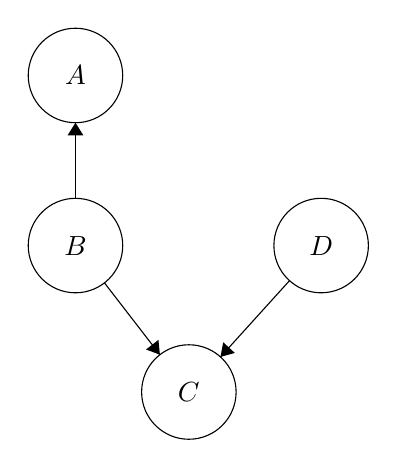
\begin{tikzpicture}[scale=0.2]
		\tikzstyle{every node}+=[inner sep=0pt]
		\draw [black] (27.3,-12.9) circle (3);
		\draw (27.3,-12.9) node {$A$};
		\draw [black] (27.3,-23.7) circle (3);
		\draw (27.3,-23.7) node {$B$};
		\draw [black] (34.5,-33) circle (3);
		\draw (34.5,-33) node {$C$};
		\draw [black] (42.9,-23.7) circle (3);
		\draw (42.9,-23.7) node {$D$};
		\draw [black] (29.14,-26.07) -- (32.66,-30.63);
		\fill [black] (32.66,-30.63) -- (32.57,-29.69) -- (31.78,-30.3);
		\draw [black] (40.89,-25.93) -- (36.51,-30.77);
		\fill [black] (36.51,-30.77) -- (37.42,-30.52) -- (36.68,-29.84);
		\draw [black] (27.3,-20.7) -- (27.3,-15.9);
		\fill [black] (27.3,-15.9) -- (26.8,-16.7) -- (27.8,-16.7);
		\end{tikzpicture}
		\caption{Second Bayesian network that is a perfect map of $P$}
		\label{fig:bayesian_perfect_map_equivalent}
  \end{figure}

  \item We can draw the minimal I-map for $P$ as a Markov network as shown in Figure \ref{fig:markov_network} by moralizing our perfect map from before.

  \begin{figure}[!h]
  	\centering
  	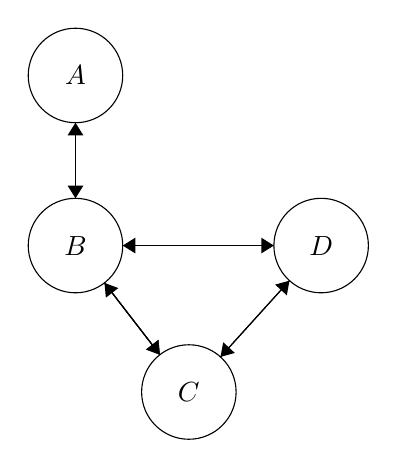
\begin{tikzpicture}[scale=0.2]
			\tikzstyle{every node}+=[inner sep=0pt]
			\draw [black] (27.3,-12.9) circle (3);
			\draw (27.3,-12.9) node {$A$};
			\draw [black] (27.3,-23.7) circle (3);
			\draw (27.3,-23.7) node {$B$};
			\draw [black] (34.5,-33) circle (3);
			\draw (34.5,-33) node {$C$};
			\draw [black] (42.9,-23.7) circle (3);
			\draw (42.9,-23.7) node {$D$};
			\draw [black] (29.14,-26.07) -- (32.66,-30.63);
			\fill [black] (32.66,-30.63) -- (32.57,-29.69) -- (31.78,-30.3);
			\draw [black] (40.89,-25.93) -- (36.51,-30.77);
			\fill [black] (36.51,-30.77) -- (37.42,-30.52) -- (36.68,-29.84);
			\draw [black] (27.3,-20.7) -- (27.3,-15.9);
			\fill [black] (27.3,-15.9) -- (26.8,-16.7) -- (27.8,-16.7);
			\draw [black] (27.3,-15.9) -- (27.3,-20.7);
			\fill [black] (27.3,-20.7) -- (27.8,-19.9) -- (26.8,-19.9);
			\draw [black] (29.14,-26.07) -- (32.66,-30.63);
			\fill [black] (32.66,-30.63) -- (32.57,-29.69) -- (31.78,-30.3);
			\draw [black] (32.66,-30.63) -- (29.14,-26.07);
			\fill [black] (29.14,-26.07) -- (29.23,-27.01) -- (30.02,-26.4);
			\draw [black] (36.51,-30.77) -- (40.89,-25.93);
			\fill [black] (40.89,-25.93) -- (39.98,-26.18) -- (40.72,-26.86);
			\draw [black] (39.9,-23.7) -- (30.3,-23.7);
			\fill [black] (30.3,-23.7) -- (31.1,-24.2) -- (31.1,-23.2);
			\draw [black] (30.3,-23.7) -- (39.9,-23.7);
			\fill [black] (39.9,-23.7) -- (39.1,-23.2) -- (39.1,-24.2);
			\end{tikzpicture}
		\caption{Minimal I-map Markov network of $P$}
		\label{fig:markov_network}
 	\end{figure}

 	We simply make all edges undirected and marry the parents of $C$. This is because we know that any edge in $G$ must exists in $G'$ (since otherwise we would be introducing new independences between those two variables). However, we note that in $G$ we have $B \not\perp D \mid C$, and therefore, we must introduce an edge between $B$ and $D$ (the parents of $C$) in order to make sure the network does not introduce a false independence.

 	However, from the above, we immediately realize that this is not a perfect map since by introducing the edge between $D$ and $B$, we now lose the information that $B \perp D$ as given in $P$. Therefore $G'$ cannot be a perfect map since $I(G') \subset I(P)$.
\end{enumerate}


\pagebreak
\section*{Problem 2}

\begin{enumerate}[label=(\alph*)]
\item We can decide if $(C \perp D), (C \perp B) \in I(P)$ by checking based on the probabilites. If $C \perp D$, we must have $P(C,D) = P(C)P(D)$ and if $C \perp B$ we must have $P(C,B) = P(C)P(B)$. Since we're given the full joint distributions, it is easy enough to calculate each of the marginals. We have:
\begin{align*}
&P(C = 1) = \sum_{a,b,d} P(A = a, B=b, C=1, d=d) &= \frac{1}{2}\\
&P(C = 0) &= \frac{1}{2} \\
&P(B = 1) =\sum_{a,c,d} P(A = a, B=1, C=c, d=d) &= \frac{5}{8} \\
&P(B = 0) &= \frac{3}{8} \\
&P(D = 1) =\sum_{a,b,c} P(A = a, B=b, C=c, d=1)&= \frac{1}{2} \\ 
&P(D = 0) &= \frac{1}{2} \\ 
&P(C = 1, D = 1) = \sum_{a,b} P(A = a, B=b, C=1, d=1) &= \frac{1}{4} \\
&P(C = 1, D = 0) = \sum_{a,b} P(A = a, B=b, C=1, d=0) &= \frac{1}{4} \\
&P(C = 0, D = 1) = \sum_{a,b} P(A = a, B=b, C=0, d=1) &= \frac{1}{4} \\
&P(C = 0, D = 0) &= \frac{1}{4} \\
&P(C = 1, B = 1) =\sum_{a,c,d} P(A = a, B=1, C=1, d=d) &= \frac{1}{4} \\
&P(C = 1, B = 0) =\sum_{a,c,d} P(A = a, B=0, C=1, d=d) &= \frac{3}{8} \\
&P(C = 0, B = 1) =\sum_{a,c,d} P(A = a, B=1, C=0, d=d) &= \frac{1}{4} \\
&P(C = 0, B = 0) &= \frac{1}{8} 
\end{align*}
From the above, we can immediately verify the following:
\begin{align*}
\forall c \in \{0,1\},d \in \{0,1\}: P(C =c, D=d) &= P(C=c)P(D=d) \\
\exists c \in \{0,1\},d \in \{0,1\}: P(C = c, B =b) \neq P(C = c) P(B = b) \\
\end{align*}

Therefore we can safely conclude that $C \perp D$ but $C \not\perp B$.

\item We give the solution in Figure \ref{fig:directed_result}.
\begin{figure}
	\centering
	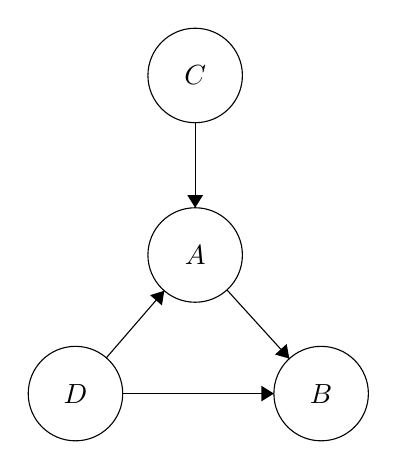
\begin{tikzpicture}[scale=0.2]
		\tikzstyle{every node}+=[inner sep=0pt]
		\draw [black] (34.6,-28.5) circle (3);
		\draw (34.6,-28.5) node {$A$};
		\draw [black] (27,-37.3) circle (3);
		\draw (27,-37.3) node {$D$};
		\draw [black] (34.6,-17.1) circle (3);
		\draw (34.6,-17.1) node {$C$};
		\draw [black] (42.6,-37.3) circle (3);
		\draw (42.6,-37.3) node {$B$};
		\draw [black] (34.6,-20.1) -- (34.6,-25.5);
		\fill [black] (34.6,-25.5) -- (35.1,-24.7) -- (34.1,-24.7);
		\draw [black] (36.62,-30.72) -- (40.58,-35.08);
		\fill [black] (40.58,-35.08) -- (40.41,-34.15) -- (39.67,-34.82);
		\draw [black] (30,-37.3) -- (39.6,-37.3);
		\fill [black] (39.6,-37.3) -- (38.8,-36.8) -- (38.8,-37.8);
		\draw [black] (28.96,-35.03) -- (32.64,-30.77);
		\fill [black] (32.64,-30.77) -- (31.74,-31.05) -- (32.49,-31.7);
	\end{tikzpicture}
	\caption{Bayesian net with directed edges for $P$ filled in.}
	\label{fig:directed_result}
\end{figure}


From (a) above, we now that $C \perp D$. This necessarily implies that $C \to A \leftarrow D$, since this is the only structure where on $A,C,D$ such that $C \perp D$. From (a), we also know that $C \not\perp B$, and therefore, we must have $C \to A \to B$ (because we must already have $C \to A$ and $D \to A$ blocks using $D$ in the path to $B$, therefore $A \to B$ must exists in order for $C \not\perp B$ to be true). Finally, given that result, $C \perp D$ must necessarily implies that $D \to B$ is the direction of the edge between $D$ and $B$ -- otherwise, we would have the path $C \to A \to B \to D$ which would contradict $C \perp D$.

The solution presented above is unique, since there are no equivalent $I$-maps due to the v-structures at $A$ and $B$ which use all the edges in the graph.

\item We now give the CPDs of each of the nodes in graph specified in (b). From the graph, we have $P(A,B,C,D) = P(C)P(D)P(A \mid D,C)P(B\mid A,D)$. From previous work, we immediately have (just by looking at the joint):
\begin{align*}
&P(C = 0) &= \frac{1}{2} \\
&P(C = 1) &= \frac{1}{2} \\
&P(D = 0) &= \frac{1}{2} \\
&P(D = 1) &= \frac{1}{2} \\
&P(A = 1\mid C = 0,D = 0) &= \frac{1}{2} \\
&P(A = 0\mid C = 0,D = 0) &= \frac{1}{2} \\
&P(A = 1\mid C = 0,D = 1) &= 0 \\
&P(A = 0\mid C = 0,D = 1) &= 1 \\
&P(A = 1\mid C = 1,D = 0) &= 1 \\
&P(A = 0\mid C = 1,D = 0) &= 0 \\ 
&P(A = 1\mid C = 1,D = 1) &= 1 \\
&P(A = 0\mid C = 1,D = 1) &= 0 \\
&P(B = 1\mid A = 0,D = 0) &= 0 \\
&P(B = 0\mid A = 0,D = 0) &= 1 \\
&P(B = 1\mid A = 0,D = 1) &= 1 \\
&P(B = 0\mid A = 0,D = 1) &= 0 \\
&P(B = 1\mid A = 1,D = 0) &= 1 \\
&P(B = 0\mid A = 1,D = 0) &= 0 \\ 
&P(B = 1\mid A = 1,D = 1) &= 0 \\
&P(B = 0\mid A = 1,D = 1) &= 1 \\
\end{align*}

Which we can verify to be correcy by simply multiplying out the conditionals given the network we stated, so we have that $P(A,B,C,D) = P(C)P(D)P(A \mid D,C)P(B \mid A, D)$:
\begin{align*}
P(A= 0, B = 0, C =0, D = 0) & = \frac{1}{2} \cdot \frac{1}{2} \cdot \frac{1}{2} \cdot 1 &= \frac{1}{8} \\
P(A= 1, B = 1, C =0, D = 0) & = \frac{1}{2} \cdot \frac{1}{2} \cdot \frac{1}{2} \cdot 1 &= \frac{1}{8} \\
P(A= 1, B = 1, C =1, D = 0) & = \frac{1}{2} \cdot \frac{1}{2} \cdot 1 \cdot 1 &= \frac{1}{8} \\
P(A= 0, B = 1, C =0, D = 1) & = \frac{1}{2} \cdot \frac{1}{2} \cdot 1 \cdot 1 &= \frac{1}{8} \\
P(A= 1, B = 0, C =1, D = 1) & = \frac{1}{2} \cdot \frac{1}{2} \cdot 1 \cdot 1 &= \frac{1}{8}
\end{align*}
\end{enumerate}


\pagebreak
\section*{Problem 3}

\begin{enumerate}[label=(\alph*)]
\item We compute the marginal conditional probability of a single value. First, for succintness, let $h_{-i} \in \{0,1\}$ represents $h_1 \in \{0,1\}, \cdots, h_{i-1} \in \{0,1\}, h_{i+1}\in \{0,1\} \cdots h_n \in \{0,1\}$ (we consider all possible values except $i$).
\begin{align*}
P(h_i \mid v) &= \frac{\sum_{h_{-i} \in \{0,1\}} P(\textbf{h}, \textbf{v})}{\sum_{h_1 \in \{0,1\}, \cdots h_n \in \{0,1\}} P(\textbf{h}, \textbf{v})} \\
&= \frac{\frac{1}{Z}\sum_{h_{-i} \in \{0,1\}} \exp\{-\alpha^T\textbf{v} - \beta^T \textbf{h} - \textbf{v}^TW\textbf{h}\}}{\frac{1}{Z}\sum_{h_1 \in \{0,1\}, \cdots h_n \in \{0,1\}} \exp\{-\alpha^T\textbf{v} - \beta^T \textbf{h} - \textbf{v}^TW\textbf{h}\}} \\
&= \frac{\exp\{-\alpha^T \textbf{v}\}\sum_{h_{-i} \in \{0,1\}} \exp\{- \beta^T \textbf{h} - \textbf{v}^TW\textbf{h}\}}{\exp\{-\alpha^T \textbf{v}\}\sum_{h_1 \in \{0,1\}, \cdots h_n \in \{0,1\}} \exp\{- \beta^T \textbf{h} - \textbf{v}^TW\textbf{h}\}} \\
&= \frac{\sum_{h_{-i} \in \{0,1\}} \exp\{- \beta^T \textbf{h} - \textbf{v}^TW\textbf{h}\}}{\sum_{h_1 \in \{0,1\}, \cdots h_n \in \{0,1\}} \exp\{- \beta^T \textbf{h} - \textbf{v}^TW\textbf{h}\}} \\
&= \frac{\sum_{h_{-i} \in \{0,1\}} \exp\{\sum_{j = 1 }^n (-\beta_j h_j - \textbf{v}^TW_jh_j)\}}{\sum_{h_1 \in \{0,1\}, \cdots h_n \in \{0,1\}} \exp\{\sum_{j = 1 }^n (-\beta_j h_j - \textbf{v}^TW_jh_j)\}} \\
&= \frac{\exp\{-\beta_i h_i - \textbf{v}W_ih_i\}\sum_{h_{-i} \in \{0,1\}} \exp\{\sum_{i \neq j } (-\beta_j h_j - \textbf{v}^TW_jh_j)\}}{\sum_{h_i \in \{0,1\}}\exp\{-\beta_i h_i - \textbf{v}W_ih_i\} \sum_{h_{-i} \in \{0,1\}} \exp\{\sum_{i \neq j} (-\beta_j h_j - \textbf{v}^TW_jh_j)\}} \\
&= \frac{\exp\{-\beta_i h_i - \textbf{v}^TW_ih_i\}}{\sum_{h_i \in \{0,1\}}\exp\{-\beta_i h_i - \textbf{v}^TW_ih_i\}} \\
&= \frac{\exp\{-\beta_i h_i - \textbf{v}^TW_ih_i\}}{1 + \exp\{-\beta_i - \textbf{v}^TW_i\}}
\end{align*}

With the above simplifcation, we note that computing $P(h_i \mid \textbf{v})$ is tractable. It consists simply of computing $-\beta_i - \textbf{v}^TW_i$, which takes $O(m)$ time, and plugging the result into the above formula.
\item We can express the conditional distributions in a compact forms as follows:
\begin{align*}
p(\textbf{h} \mid \textbf{v}) &= p(h_1 \mid \textbf{v})p(h_2 \mid h_1, \textbf{v}) \cdots p(h_n \mid h_1, \cdots h_{n-1}, \textbf{v}) \\
&= p(h_1 \mid \textbf{v})p(h_2 \mid \textbf{v})) \cdots p(h_n \mid \textbf{v})) \\
&= \prod_{i=1}^{n} p(h_i \mid \textbf{v}))
\end{align*}
This is because the network structure is a bipartite graph. Therefore, we have that $h_i \perp h_j \mid \textbf{v}$ for $i \neq j$, which allows us to simplify greatly.
\item Yes, $\sum_{h} \exp(\phi(v,h))$ can be computed efficiently. This is because
\begin{align*}
\exp\{\phi(\textbf{v}, \textbf{h})\} &= \exp\{-\alpha^T\textbf{v})\} \exp\{-\beta^T\textbf{h})\} \exp\{-\textbf{v}^W\textbf{h})\} \\
&= \prod_{i=1}^m \exp\{-\alpha_iv_i)\} \prod_{j=1}^n \exp\{-\beta_jh_j)\}\prod_{i,j} \exp\{-v_iW_{i,j}h_j)\}
\end{align*}
Therefore, we can push the sum into only the factors that are affected by it. For example:
\begin{align*}
&\sum_{h_1 \in \{0,1\}}\cdots\sum_{h_n \in \{0,1\}} \prod_{i=1}^m \exp\{-\alpha_iv_i)\} \prod_{j=1}^n \exp\{-\beta_jh_j)\}\prod_{i,j} \exp\{-v_iW_{i,j}h_j)\} \\ &= \exp\{-\alpha^T \textbf{v}\} \sum_{h_1 \in \{0,1\}} \exp\{-\beta_1 h_1 - \textbf{v}^TW_1h_1\} \cdots \sum_{h_n \in \{0,1\}} \exp\{-\beta_n h_n - \textbf{v}^TW_nh_n\} 
\end{align*}

\item Yes, for a similar reason as above (we can factorize the joint distribution and push the sums inside).
\item No. If we consider the sum-product algorithm, computing the normalizing constant would be exponenential since the size of the largest clique in any of the induced graphs is always either $m$ or $n$. WLOG, suppose we attempt to marginalize out $h_i$. Then we will introduce a new factor $\phi$ which connects all of $v_i$ with each other. This immediately introduces a clique of size $m$, and therefore, we will have an exponential algorith.
\end{enumerate}

\pagebreak
\section*{Problem 4}

We can compute this directly. WLOG, we re-label the edges such that $x_1 \to x_n$ is the newly added edge to form $G'$. We also denote $\circ$ as the vector concatenation operator. We show a step by step derivation of the inequality:
\begin{align*}
\max_{\theta'} \ell_{G'}(\theta';\mathcal{D}) &\stackrel{?}{=} \max_{\theta} \ell_{G}(\theta;\mathcal{D}) \\
\sum_{i=1}^n \sum_{\textbf{u}_i' \in Val(Pa(X_n'))}\sum_{x_i} M[x_i, \textbf{u}_i'] \log\frac{M[x_i, \textbf{u}_i']}{M[\textbf{u}_i']}  &\stackrel{?}{=} \sum_{i=1}^n \sum_{\textbf{u}_i \in Val(Pa(X_n))}\sum_{x_i} M[x_i, \textbf{u}_i] \log\frac{M[x_i, \textbf{u}_i]}{M[\textbf{u}_i]} \tag{Using $\frac{M[x_i, \textbf{u}_i]}{M[\textbf{u}_i]} = \arg\max_{\theta} \ell_{G}(\theta;\mathcal{D})$ and definition of $\ell(\cdot)$} \\
\sum_{\textbf{u}_n' \in Val(Pa(X_n'))}\sum_{x_n} M[x_n, \textbf{u}_n'] \log\frac{M[x_n, \textbf{u}_n']}{M[\textbf{u}_n']}  &\stackrel{?}{=} \sum_{\textbf{u}_n \in Val(Pa(X_n))}\sum_{x_n} M[x_n, \textbf{u}_n] \log\frac{M[x_n, \textbf{u}_n]}{M[\textbf{u}_n]} \tag{All values for $i \neq n$ are the same since parents are the same} \\
\sum_{x_n}\sum_{\textbf{u}_n \circ [x_1] \in Val(Pa(X_n) \circ [x_1])} M[x_n, \textbf{u}_n \circ [x_1]] \log\frac{M[x_n, \textbf{u}_n \circ [x_1]]}{M[\textbf{u}_n \circ [x_1]]}  &\stackrel{?}{=}\sum_{x_n} \sum_{\textbf{u}_n \in Val(Pa(X_n))} M[x_n, \textbf{u}_n] \log\frac{M[x_n, \textbf{u}_n]}{M[\textbf{u}_n]} \tag{re-order and expand sums} \\
\sum_{x_n}\sum_{\textbf{u}_n \in Val(Pa(X_n))} \sum_{x_1} M[x_n, \textbf{u}_n \circ [x_1]] \log\frac{M[x_n, \textbf{u}_n \circ [x_1]]}{M[\textbf{u}_n \circ [x_1]]}  &\stackrel{?}{=} \sum_{x_n}\sum_{\textbf{u}_n \in Val(Pa(X_n))} M[x_n, \textbf{u}_n] \log\frac{M[x_n, \textbf{u}_n]}{M[\textbf{u}_n]} \tag{sum over $x_1$}
\end{align*}
From the above, we focus just on the inner most sum on the LHS and note the following:
\begin{align*}
M[x_n, \textbf{u}_n \circ [x_1]] \geq 0 \\
M[\textbf{u}_n \circ [x_1]] \geq 0 \\
\sum_{x_1} M[x_n, \textbf{u}_n \circ [x_1]] &= M[x_n, \textbf{u}_n] \\
\sum_{x_1} M[\textbf{u}_n \circ [x_1]] &= M[\textbf{u}_n] \\
\implies \sum_{x_1}M[x_n, \textbf{u}_n \circ [x_1]] \log \frac{M[x_n, \textbf{u}_n \circ [x_1]]}{M[\textbf{u}_n]} &\geq M[x_n, \textbf{u}_n ] \log \frac{M[x_n, \textbf{u}_n ]}{M[\textbf{u}_n]} ]] \tag{by the log sum inequality}
\end{align*}
Given the above, we note that the original LHS must be larger than or equal to the original RHS, and so we conclude:
$$
\max_{\theta'} \ell_{G'}(\theta';\mathcal{D}) \geq \max_{\theta} \ell_{G}(\theta;\mathcal{D})
$$

\pagebreak
\section*{Problem 5}

Note that we modified the starter code to ``actually'' do cross validation only 10 times :)
\begin{enumerate}[label=(\alph*)]
\item For the Naive Bayes Classifier, 10-fold cross validation total test accuracy is 0.9181 on 232 examples, which gives a test error of 0.0819.
\item For the Tree Augmented Naive Bayes Classifer, 10-fold cross validation total test accuracy is 0.9698 on 232 examples, which gives a test error of 0.0302.
\item We can evaluate on the missing data by marginalizing the unknown variables as described in the problem. In this case, the Naive Bayes models gives a $97.73\%$ chance to label being Democrat. The TABN classifier on the other hand gives a $100\%$ chance. Furthermore, it is simple to calculate $P(A_{12} \mid A_{observed})$. We simply have:
$$
P(A_{12} \mid A_{observed}) = \frac{\sum_{a_{-observed}, c}P(A_1, \cdots, A_{16}, C)}{\sum_{a_{-observed},c,a_{12}}P(A_1, \cdots, A_{16}, C)}
$$

Prediting vote of A12 using NBClassifier on missing data as $P(A_{12}=1|A_{observed}) = 0.1416$ using Naive Bayes and prediting vote of A12 using TANBClassifier on missing data as $P(A_{12}=1|A_{observed}) = 0.1024$.

\item Naive Bayes (Small Data) 10-fold cross validation total test accuracy is 0.9009 on 232 examples. However, TANB Classifier (Small Data) 10-fold cross validation total test accuracy is 0.8534 on 232 examples. The reason why the test error on the TABN might be higher than the test error on the Naive Bayes is because the TANB is a more complex model, and was therefore better able to fit the training data distribution. In this case, since the training data was quite small, this led to overfitting, leading to poorer performance on the test set. On the other hand, the Naive Bayes did not overfit as much (due to its more limited model capacity), and was therefore able to perform better on the test set.
\end{enumerate}


\end{document}
